\chapter{The Design and Development of the Immotion Exergame}\label{chapter:implementation}

This chapter outlines the design and development of the Immotion exergame for warm up routine guidance and motivation. We begin this chapter with the description of the design methodology used for the development. For the purpose of this thesis, an iterative and prototype driven, user centred design methodology was adopted. After the methodology has been introduced, we continue with the in depth discussion of each individual development phase. Our main focus is placed on the last two stages of the development process in which we develop the prototype and the final version of our exergame solution, and evaluate them utilizing various qualitative and quantitative evaluation methods. During all the development phases, the particular needs of individuals who engage in physical (sports) activities but rarely or never warm up prior to them have been taken into account and gathered through the adopted design process in order to make an adequate exergame for warm up guidance and motivation. %We chose the \textit{Spiral model}s as our chosen exergame development model.  

\section{Overview of User Centered Design}
\gls{ucd} represents \textit{a user interface design process} that puts its focus on usability goals, explicit understanding of users, environment, and tasks to be performed \cite{ucd2}. Moreover, it is an iterative process, where design and evaluation phases are included from the first stage of the development, that addresses the whole user experience, and is driven and refined by user-centered evaluation. %Shawn Lawton Henry and Mary Martinson, Accessibility in User-Centered Design + https://www.w3.org/WAI/redesign/ucd + https://www.usability.gov/what-and-why/user-centered-design.html
Adopted from \cite{userCenteredDesign}, the following are the general and advised phases of the \acrshort{ucd} process:
\begin{itemize}
\item \textit{Specify the context of use}. Identify future users of the solution, the intended purpose of usage, and the conditions under which the solution will be used.
\item \textit{Specify requirements}. Identify user goals that must be met in order for the solution success.
\item \textit{Create design solutions}. Done in stages, building from a rough concept to a complete and final design.
\item \textit{Evaluate designs}. Evaluation should be performed through usability testing with actual users.
\end{itemize}
Even though being a relatively new field, exergame developers often indicate the relevance of including the players in the design process and point out the benefits of adopting \acrshort{ucd} in exergames development. In their study on exergame design for elderly users, Gerling and Masuch recommend and utilize \acrshort{ucd} for developing exergames for an elderly audience \cite{webster2014systematic}. Researchers in \cite{hernandez2013designing} also take advantage of \acrshort{ucd} in their year long study whilst developing action-oriented exergames for children with cerebral palsy. As showed that \acrshort{ucd} can be used for designing effective exergames for specific target demographic, we also adopt this approach in the development of our exergame solution.
\section{The Context of Use}
There exist commercial and non-commercial exergame solutions designed to encourage physical activity. These solutions are mainly intended to be used for home and in-door workout activities. Many of them offer multitudes of predefined exercise programs and also make it easy to create a fully customized workout plan that are suited for individual's needs and abilities. However, in our research, we found no available solutions that focus solely on the warm up routine as a preparatory activity before physically more demanding exercise. Taking this into account, as well as the fact that warm up routines are crucial part of any sports activity \cite{bishop2003warm1,shellock1985warming} although often avoided by multitude of athletes \cite{fradkin2006does}, with the Immotion exergame we chose to tackle exactly this issue. We design and develop our exergame to be used as a warm up guidance and motivation tool. That is, our exergame is intended to be used in gyms and fitness centres before any arduous sports activity. Additionally, we target individuals, above all amateur athletes, who often avoid or do not know how to perform a proper warm up routine. Lastly, we design our exergame so the movements required to be executed are intuitive for  the player and do not require additional explanation nor previous exercise knowledge. \pagebreak
\section{Overview of the Development Phases}
The development of the Immotion exergame consisted of three phases which are according to the well accepted \acrshort{ucd} development phases outlined in the previous section and depicted in Figure \ref{fig:iterations}: 
\begin{itemize}
\item Requirements gathering 
\item First prototype development with user evaluation
\item Final exergame development with further user evaluation
\end{itemize}
In the following sections, each iteration presented in \textit{Development} slice and the \textit{Requirement Gathering} iteration of the \textit{Planning} slice depicted in Figure \ref{fig:iterations} will be further detailed. 
\begin{figure}[h]
    \centering
    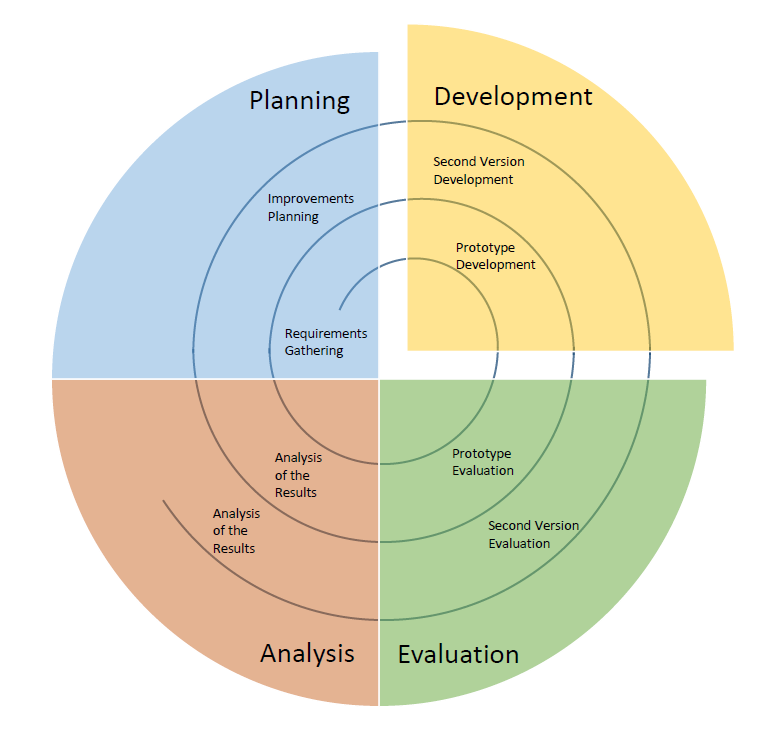
\includegraphics[width=0.9\textwidth]{iterations}
    \caption{Overview of the development iterations}
    \label{fig:iterations}
\end{figure}
\section{Requirements Gathering}
This iteration was an exploratory step that justified the development and identified the currently available solutions in the domain of exergames for warm up before sports activities. This was achieved through initial literature review related to exergame, gamification, and motivational psychology which identified the most important areas to be addressed when developing gamified solution in the given context. Furthermore, in order to design an enjoyable exergame solution, several warm up and sports related requirements needed to be considered too. Having this in mind, sports and fitness related literature have been reviewed as well. Particular attention has been put on those warm up exercises that could hypothetically help in injury prevention and improve performance. Our exergame is meant to be used in gym or fitness centers before physically demanding sports activities. Hence, the movements required in the game should be those that increase core body temperature, blood flow, and prepare the body for the subsequent exercise. In addition, we had to take into account certain constraints and requirements when selecting these movements. Some of the them were as follows:
\begin{itemize}
\item Movements needed to be easily detectable by only one Kinect device.
\item Movements should be easy enough to be correctly performed without any prior knowledge of the movement or exercise.
\item Only movements that can be executed without additional equipment should be considered.   
\item Only movements recommended for the general warm up routines outlined in sports related literature and suggested by experts should be considered.
\item The duration of the exergame guided warm up routine should correspond to the warm up duration suggested by sports literature and experts.
\end{itemize}
%http://assets.ngin.com/attachments/document/0035/1162/FIFA_11__EXERCISES.pdf
%https://www.kort.com/uploadedFiles/KORT/Content/Services/Sports_Medicine/Concussion_Management/FIFA-the-11-Booklet.pdf
Since no well documented and medically supported warm up programmes for workout routines were found,  the required movements were adopted from the 
\gls{fifa} \cite{fifa} warm up programme which mostly focuses on core and leg strength, balance, and agility. These programmes were shown to have significant impact on injury reduction in football players and can lead to improvements in thigh muscle strength, jump height, and sprint speed \cite{silvers2015efficacy}. %https://www.ncbi.nlm.nih.gov/pmc/articles/PMC4245655/
Based on the mentioned warm up programs review, the previously listed requirements, and hardware restrictions outlined, the following movements were found to be suitable for the prototype solution: \textit{jump right}, \textit{jump left}, \textit{jump up}, and \textit{squat}.\\
After the requirements were specified and the required movements selected, we continued with the prototype development phase.
